% Chapter 1

\chapter{Theory of Single-Particle Beam Dynamics in the Large Hadron Collider} % Main chapter title

\label{Chapter1} % For referencing the chapter elsewhere, use \Cref{Chapter1}

%----------------------------------------------------------------------------------------

Beam dynamics is a field of accelerator science which is significant for the design, operation, performance, and protection of an accelerator. 
In this section an overview is given of the theories of beam dynamics which are relevant to the material presented in this thesis.
The chapter begins with a description of the linear dynamics, then progresses to deal with aspects of the non-linear dynamics, concluding with a discussion of the luminosity.

%----------------------------------------------------------------------------------------

\section{Linear Beam Dynamics}

Define concept: bend and focus particles to have them remain within the aperture tolerance of the machine.
Bend with dipoles, focus with quadrupoles typically.
% Within the linear approximation, non-linear magnetic fields are ignored and the beam dynamics is described by linear differential equations.
\Cref{fig:frenet_system} illustrates the Frenet-Serret coordinate system traditionally used in linear beam dynamics.
\bigbreak

\begin{figure}[!htb]
    \begin{center}
    
\includegraphics[width = 0.7\linewidth]{Figures/placeholder.png}
    \caption{Coordinate system for linear accelerator optics.}
    \label{fig:frenet_system}
    \end{center}
\end{figure}

Coordinate system travels longitudinally with the particle, along a reference trajectory defined by an "ideal" / "reference" / "synchronous" particle.
Define $s$ as longitudinal / curvilinear coordinate.
Define $\rho(s)$ local radius of curvature (depends on $\mathbf{B}$ and varies along ring).
Define $(x, x\prime, y, y\prime)$, coordinates of transverse phase space:
$x$ and $y$ are particle coordinates in the transverse planes (transverse displacement).
$x^{'}$ and $y^{'}$ are "divergent angles" (says Ewen) in the $x$ and $y$ plane (differentiation with respect to $s$).
\bigbreak

In linear regime, dipoles define ideal orbit for particle of \emph{reference momentum} $p_0$.
Ideal orbit goes through magnetic center of all elements and comes back on itself after a revolution, and is called a \emph{closed orbit}.
In practice dipolar errors (and more) will distort the real closed orbit from the ideal designed orbit.
Particles within the beam are distributed in amplitude (the beam occupies a finite area in $(x, x\prime, y, y\prime)$ phase space). 
The closed orbit defines the path of a particle with zero amplitude within the beam.
In practice particles oscillate around the closed orbit because of the focusing forces. 
In the LHC this focusing is provided predominantly by quadrupole magnets.
\bigbreak

From Ewen: quadrupolar fields acting on charged particles displaced from the central axis provide a restoring (focusing) force proportional to the displacement in one transverse plane, while simultaneously providing a divergent (defocusing) force in the other. 
Tradition: a quadrupole focusing in the horizontal plane and defocusing in the vertical is referred to as a \emph{focusing quadrupole}. 
A quadrupole defocusing in the horizontal plane but focusing in the vertical is referred to as a \emph{defocusing quadrupole}.
An alternating arrangement of focusing and defocusing quadrupoles, referred to as a $\mathrm{FODO}$ lattice, can create a net focusing in both planes [ref 18 Ewen]. 
\Cref{fig:dipole_quadrupole_fields} illustrates magnetic fields in an idealized dipole and quadrupole, together with the forces exerted on a positively charged particle travelling into the page.
\bigbreak

\begin{figure}[!htb]
    \begin{center}
    
\includegraphics[width = 0.9\linewidth]{Figures/placeholder.png}
    \caption{Magnetic fields and forces in an idealized dipole (having a $cos(\phi)$ current distribution in the circular coil) and an idealized focusing quadrupole (having a $cos(2\phi)$ current distribution in the circular coil). Current in the dipole and quadrupole coils are indicated in colour. Forces exerted by the magnet on a positive charge travelling into the page are illustrated. Adapted from [19].}
    \label{fig:dipole_quadrupole_fields}
    \end{center}
\end{figure}

In circular machine focusing from quads is periodic in $s$ with a period of max the circumference of the machine.
Motion in the transverse plane is described by Hill’s equation, \cref{eq:hill_equation}, where $k(s)$ is a periodic coefficient describing the restoring force due to the distribution of focusing fields around the ring.
\bigbreak

\begin{equation}
    u^{\prime \prime} \pm k(s) u = 0; \quad u = x, y; \quad u^{\prime} = \frac{\mathrm{d}u}{\mathrm{d}s}
    \label{eq:hill_equation}
\end{equation}
\bigbreak

Solutions to Hill’s equation take the form of \cref{eq:hill_solution},
\bigbreak

\begin{equation}
    \begin{aligned}
    x &= \sqrt{\beta_{x}(s) \epsilon_{x}} \cos \left(\phi_{x}(s) + \phi_{x_0}\right) \\
    y &= \sqrt{\beta_{y}(s) \epsilon_{y}} \cos \left(\phi_{y}(s) + \phi_{y_0}\right)
    \end{aligned}
    \label{eq:hill_solution}
\end{equation}

where $\epsilon$ is the emittance of a particle and is a constant of the motion at a given energy.
$\beta(s)$ is called the \emph{beta-function} and describes the variation of the oscillation envelope around the ring. 
In particle colliders such as the LHC, it is usual to denote the beta-functions at the Interaction Points (where the beams are made to collide) as \betastar.
\bigbreak

Particles oscillate around the ring, \emph{betatron oscillations}, and the number of oscillations around the ring is the \emph{tune}, $Q_{x,y}$.
The tune is defined in \cref{eq:tune_definition}, where $\Delta \phi_{x, y}$ is the total betatron phase advance undergone by a particle during one revolution around the accelerator ring.
\bigbreak

\begin{equation}
    Q_{x, y} = \frac{1}{2 \pi} \Delta \phi_{x, y} = \frac{1}{2 \pi} \oint \frac{\mathrm{d}s}{\beta_{x, y}(s)}
    \label{eq:tune_definition}
\end{equation}

\Cref{fig:particle_trajectories} shows a tracking simulation of a particle undergoing such betatron oscillations in the LHC Arc12.
Dipole errors were added which have distorted the closed orbit away from the ideal path.
\bigbreak

\begin{figure}[!htb]
    \begin{center}
    
\includegraphics[width = 0.7\linewidth]{Figures/placeholder.png}
    \caption{Tracking simulation in LHC Arc12 of a particle undergoing betatron oscillations.}
    \label{fig:particle_trajectories}
    \end{center}
\end{figure}

Define the \emph{gamma-function} $\gamma(s)$ which describes the envelope of oscillations in $x\prime$ and $y\prime$.
Both are related by the \emph{alpha-function}:
\bigbreak

\begin{equation}
    \alpha_{x, y} = -\frac{1}{2} \frac{\mathrm{d}}{\mathrm{d}s} \beta_{x, y}(s) = \sqrt{\gamma_{x, y}(s) \beta_{x, y}(s) - 1}
    \label{eq:alpha_function}
\end{equation}
\bigbreak

In linear regime, trajectories are ellipses in phase space $(x, x\prime, y, y\prime)$.
$\alpha(s)$, $\beta(s)$, $\gamma(s)$ and $\epsilon$ define the equation of the ellipse, \cref{eq:ellipse_equation}.
\Cref{fig:phase_space_ellipse} shows a schematic illustration of the phase space ellipse.
\bigbreak

\begin{equation}
    \gamma_{u}(s) u^{2} + 2 \alpha_{u}(s) u u^{\prime} + \beta_{u}(s) z^{\prime 2} = \epsilon \quad \text { where } u = x, y
    \label{eq:ellipse_equation}
\end{equation}
\bigbreak

\begin{figure}[!htb]
    \begin{center}
    
\includegraphics[width = 0.85\linewidth]{Figures/placeholder.png}
    \caption{Phase space ellipse in the transverse $z$, $z\prime$ plane, where $z$ represents either $x$ or $y$.}
    \label{fig:phase_space_ellipse}
    \end{center}
\end{figure}

Say emittance ($\epsilon$) defines phase space ellipse area.
Liouville's theorem: phase space volume (ellipse area) is constant in a closed system.
In the LHC, protons, little synchrotron radiation [ref 20 ewen] we can consider emittance a constant (but at multi-$\mathrm{TeV}$ energy radiation emission may become non-negligible).
Acceleration -> no more Liouville and \emph{physical emittance} ($\epsilon$) will reduce with increasing energy.
One can construct \emph{normalized emittance} ($\epsilon_{\gamma}$) which is invariant with beam energy.
See \cref{eq:normalized_emittance}, where $\beta_{rel}$ and $\gamma_{rel}$ are the relativistic beta and gamma functions:
\bigbreak

\begin{equation}
    \epsilon_{\gamma} = (\beta_{\mathrm{rel}} \gamma_{\mathrm{rel}}) \epsilon
    \label{eq:normalized_emittance}
\end{equation}
\bigbreak

For a specific particle we use \emph{single particle emittance}.
Different particles may have different ones.
They will go through (undergo?) betatron oscillations of different amplitudes.
We can define \emph{beam emittance}: typically defined as the emittance corresponding $1\sigma$ amplitude in assumed Gaussian particle distribution.
\bigbreak

The phase space trajectory of a particle depends on $\alpha(s)$, $\beta(s)$, and $\gamma(s)$.
The transformation to \emph{Courant-Snyder coordinates} [ref 21 ewen] (sometimes called \emph{normalized Courant-Snyder coordinates}) removes this dependency, see \cref{eq:courant_snyder_coordinates},
\bigbreak

\begin{equation}
    \left(\begin{array}{c}
    \hat{u} \\
    \hat{u}^{\prime}
    \end{array}\right) = \left(\begin{array}{cc}
    \frac{1}{\sqrt{\beta_{u}(s)}} & \frac{\alpha_{u}(s)}{\sqrt{\beta_{u}(s)}} \\
    0 & \sqrt{\beta_{u}(s)}
    \end{array}\right)\left(\begin{array}{c}
    u \\
    u^{\prime}
    \end{array}\right) \quad \text{ where } u = x, y
    \label{eq:courant_snyder_coordinates}
\end{equation}

where the Courant-Snyder coordinates are denoted by \^{}.
In this new system particles follow circular trajectories in phase space.
\bigbreak

Say particles within the beam have a distribution in momentum, around designed momentum $p_0$.
For a particle that doesn't have $p_0$ we define the \textit{relative momentum deviation} $\delta$, \cref{eq:momentum_deviation}:
\bigbreak

\begin{equation}
    \delta = \frac{p - p_0}{p_0}
    \label{eq:momentum_deviation}
\end{equation}
\bigbreak

Define \textit{magnetic rigidity}: relates magnetic flux $\mathbf{B}$ (perpendicular to motion) with local radius of curvature and particle momentum $\mathbf{P}$.
See \cref{eq:beam_rigidity}:
\bigbreak

\begin{equation}
    \lvert \mathbf{B} \rho \rvert = \frac{\lvert \mathbf{P} \lvert}{e}
    \label{eq:beam_rigidity}
\end{equation}
\bigbreak

Say difference to $p_0$ introduce \emph{chromatic} errors into the beam dynamics.
The most important one is \emph{dispersion}.
Different momenta(um?) -> different beam rigidity -> different local radius of curvature in dipoles -> different orbit.

Deviation to reference orbit is defined by the \emph{Dispersion function}, $D(s)$ [ref 23 ewen].
In a region of non-zero dispersion the contribution to the orbit of a particle is described by \cref{eq:dispersion_contribution_to_orbit}:
\bigbreak

\begin{equation}
    \begin{aligned}
    \Delta x_{\mathrm{dispersion}} &= D_{x}(s) \delta \\
    \Delta y_{\mathrm{dispersion}} &= D_{y}(s) \delta
    \end{aligned}
    \label{eq:dispersion_contribution_to_orbit}
\end{equation}
\bigbreak

The orbit of any given particle is defined by \cref{eq:_particle_orbit}:
\bigbreak

\begin{equation}
    u = u_{\mathrm{betatronic}} + u_{\mathrm{dispersion}} + \left.u_{\mathrm{closed \ orbit}} \right\rvert_{\delta = 0}
    \label{eq:_particle_orbit}
\end{equation}

%----------------------------------------------------------------------------------------

\section{Non-Linear Magnetic Multipoles}

%----------------------------------------------------------------------------------------

\section{Formalism of Non-Linear Beam Dynamics}

%----------------------------------------------------------------------------------------

\section{Phenomenology of Non-Linear Beam Dynamics}

\subsection{Chromaticity}

\subsection{Detuning with Amplitude}

\subsection{Decoherence}

\subsection{Resonances and RDTs / CRDTs}

https://cds.cern.ch/record/1533084/files/CERN-THESIS-2013-022.pdf

%----------------------------------------------------------------------------------------

\section{Betatron Coupling}

Talk about the closest tune approach \(\Delta Q_{\mathrm{min}}\) quantity.
Without betatron coupling in the machine, horizontal and vertical tunes can be matched to the same fractional value.
In the presence of betatron coupling, the \emph{coupled fractional tunes} \(Q_1\) and \(Q_2\) cannot be matched to the same value and a minimal separation can be observed.
This separation is called the \emph{closest tune approach} and is given as the \(\Delta Q_{\mathrm{min}}\) quantity.
\Cref{fig:closest_tune_approach} shows an illustration of the phenomenon, where both the unperturbed and coupled fractional tunes are plotted against the uncoupled tune split.
The closest tune approach is the minimum distance between the two red curves, highlighted by an arrow.

\begin{figure}[!htb]
    \begin{center}
    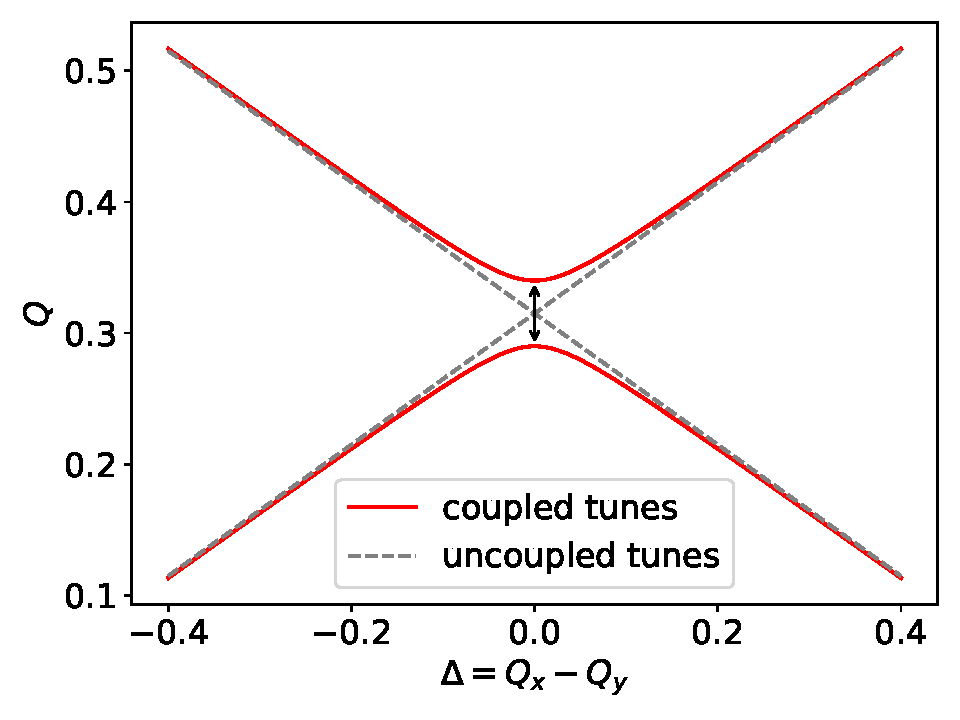
\includegraphics[width = 0.9\linewidth]{Figures/Chapter2/tune_perturbation.pdf}
    \caption{Illustration of coupled and uncoupled fractional tunes versus the uncoupled tune split.}
    \label{fig:closest_tune_approach}
    \end{center}
\end{figure}

%----------------------------------------------------------------------------------------

\section{Luminosity}

%----------------------------------------------------------------------------------------